\documentclass[12pt]{article}
\usepackage{amsmath,amsthm,amssymb,amsfonts,setspace, commath, graphicx, xfrac}

\textwidth 7.0 truein
\oddsidemargin -0.25in   %left-hand edge
\evensidemargin -0.5 truein  %right-hand edge
\topmargin -0.85in      %top of paper to top of head, pulls whole unit
\textheight 9.5in

%%%% In most cases you won't need to edit anything above this line %%%%

\begin{document}
\hfill Tanner Kvarfordt

\hfill A02052217

\hfill Assignment \#7

\begin{itemize}
\item[4.2.2)] Draw the projection of $\mathbf{b}$ onto $\mathbf{a}$ and also compute it from $\mathbf{p}=\hat{\mathbf{x}}\mathbf{a}$.
\begin{itemize}
\item[a)] $\mathbf{b}=\left[\begin{array}{c} \cos\theta \\ \sin\theta \end{array}\right]$ and 
$\mathbf{a}=\left[\begin{array}{c} 1 \\ 0 \end{array}\right]$
\item[b)] $\mathbf{b}=\left[\begin{array}{c} 1 \\ 1 \end{array}\right]$ and 
$\mathbf{a}=\left[\begin{array}{r} 1 \\ -1 \end{array}\right]$
\end{itemize}

\textit{Solution.}
\begin{itemize}
\item[a)] 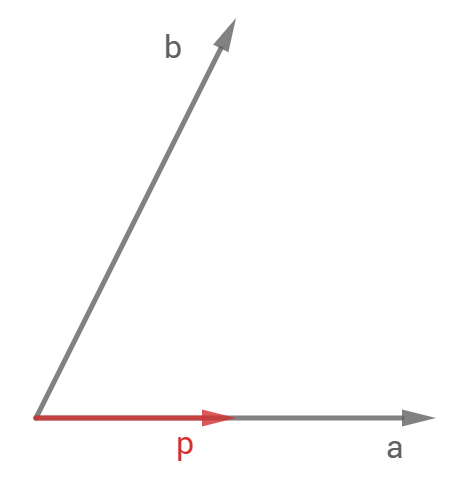
\includegraphics[scale=0.5]{a.PNG} \\
		  $\hat{\mathbf{x}}=\frac{\mathbf{a}^T\mathbf{b}}{\mathbf{a}^T\mathbf{a}}=\frac{\cos\theta}{1}=\cos\theta$, so 
	      $\mathbf{p}=\hat{\mathbf{x}}\mathbf{a}=\cos\theta\left[\begin{array}{c} 1 \\ 0 \end{array}\right]=
          \left[\begin{array}{c} \cos\theta \\ 0 \end{array}\right]$
\item[b)] 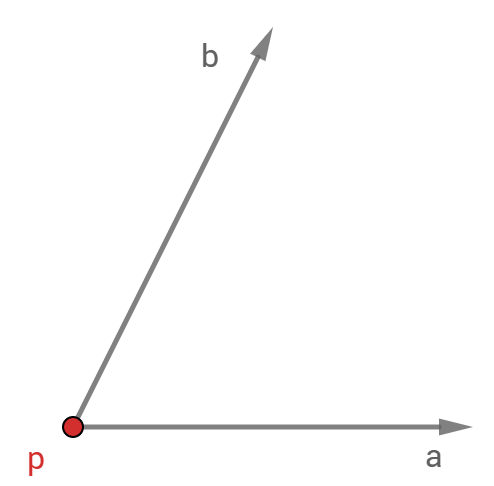
\includegraphics[scale=0.5]{b.PNG} \\
		  $\hat{\mathbf{x}}=\frac{\mathbf{a}^T\mathbf{b}}{\mathbf{a}^T\mathbf{a}}=\frac{0}{2}=0$, so 
	      $\mathbf{p}=\hat{\mathbf{x}}\mathbf{a}=0\left[\begin{array}{r} 1 \\ -1 \end{array}\right]=
          \left[\begin{array}{r} 0 \\ 0 \end{array}\right]$
\end{itemize}

\item[4.2.13)] Suppose $A$ is the 4 by 4 identity matrix with its last column removed. $A$ is 4 by 3. Project $\mathbf{b}=(1,2,3,4)$ onto the column space of $A$. What shape is the projection matrix $P$ and what is $P$?

\textit{Solution.}
\begin{itemize}
\item[a)] $A^T=
	      \left[\begin{array}{cccc} 
	      1 & 0 & 0 & 0\\
	      0 & 1 & 0 & 0\\
	      0 & 0 & 1 & 0\\
	     \end{array}\right]$, so $A^TA\hat{x}=A^T\vec{b} \Rightarrow 
         \left[\begin{array}{ccc} 
	      1 & 0 & 0 \\
	      0 & 1 & 0 \\
	      0 & 0 & 1 \\
	     \end{array}\right]\hat{x}=
         \left[\begin{array}{c} 1 \\ 2 \\ 3\end{array}\right] 
         \Rightarrow \hat{x}=\left[\begin{array}{c} 1 \\ 2 \\ 3\end{array}\right]$, \\
         so $\vec{p}=A\hat{x} \Rightarrow \vec{p}=\left[\begin{array}{c} 1 \\ 2 \\ 3\\ 0\end{array}\right]$
\item[b)] $P$ will be $4 \times 4$ since it projects a 4-D vector onto another 4-D vector. 
	      $P=\left[\begin{array}{cccc} 
	      1 & 0 & 0 & 0\\
	      0 & 1 & 0 & 0\\
	      0 & 0 & 1 & 0\\
          0 & 0 & 0 & 0
	     \end{array}\right]$
\end{itemize}

\item[4.2.17)] If $P^2=P$ show that $(I - P)^2=I - P$. When $P$ projects onto the column space of $A$, $I - P$ projects onto the $\rule{1cm}{0.15mm}$.

\textit{Solution.}
\begin{itemize}
\item[a)] $(I-P)^2=(I-P)(I-P)=(I-P)I-(I-P)P=I^2-IP-(PI-P^2)$\\
		  $=I^2-IP-PI+P^2=I-P-P+P=I-P$
\item[b)] Left nullspace of $A$.
\end{itemize}

\item[4.2.27)] The important fact that ends the section is this: \textbf{If $\mathbf{A^TAx=0}$ \textit{then} $\mathbf{Ax=0}$.} \\
\textit{New Proof:} The vector $Ax$ is in the nullspace of $\rule{1cm}{0.15mm}$. $Ax$ is always in the column space of $\rule{1cm}{0.15mm}$. To be in both of those perpendicular spaces, $Ax$ must be zero.

\textit{Solution.}
\begin{itemize}
\item[a)] $A^T$
\item[b)] $A$
\end{itemize}

\item[4.3.6)] Project $\mathbf{b}=(0,8,8,20)$ onto the line through $\mathbf{a}=(1,1,1,1)$. Find $\hat{x}=\mathbf{a}^T\mathbf{b}/\mathbf{a}^T\mathbf{a}$ and the projection $\mathbf{p}=\hat{x}\mathbf{a}$. Check that $\mathbf{e}=\mathbf{b}-\mathbf{p}$ is perpendicular to $\mathbf{a}$, and find the shortest distance $\norm{\mathbf{e}}$ from $\mathbf{b}$ to the line through $\mathbf{a}$.

\textit{Solution.}
\begin{itemize}
\item[a)] $\hat{x}=\frac{\mathbf{a}^T\mathbf{b}}{\mathbf{a}^T\mathbf{a}}=\frac{36}{4}=9$
\item[b)] $\mathbf{p}=\hat{x}\mathbf{a}=(9,9,9,9)$
\item[c)] $\mathbf{e}=\mathbf{b}-\mathbf{p}=(-9,-1,-1,11)$ and $\mathbf{e}\cdot\mathbf{a}=-9-1-1+11=0$ and thus $\mathbf{e}$ is perpendicular to $\mathbf{a}$.
\item[d)] $\norm{\mathbf{e}}=\sqrt[]{81+1+1+121}=\sqrt[]{204}=2\hspace{1mm}\sqrt[]{51}$
\end{itemize}

\item[4.3.12)] This problem projects $b=(b_1,\ldots,b_m)$ onto the line through $a=(1,\ldots,1)$. We solve $m$ equations $ax=b$ in one unknown (by least squares).
\begin{itemize}
\item[a)] Solve $a^Ta\hat{x}=a^Tb$ to show that $\hat{x}$ is the mean (the average) of the $b$'s.
\item[b)] Find $e=b-a\hat{x}$ and the variance $\norm{e}^2$ and the standard deviation $\norm{e}$.
\item[c)] The horizontal line $\hat{b}=3$ is closest to $b=(1,2,6)$. Check that $p=(3,3,3)$ is perpendicular to $e$ and find the 3 by 3 projection matrix $P$.
\end{itemize}

\textit{Solution.}
\begin{itemize}
\item[a)] $b$ is $m \times 1$, so $a^T$ must be $1 \times m$, so $a^Ta=\Sigma_{i=1}^{m}\hspace{0.5mm}1=m$. Also, $a^Tb=\Sigma_{i=1}^{m}\hspace{0.5mm}b_i$. \\
Thus, $\hat{x}=\frac{\Sigma_{i=1}^{m}\hspace{0.5mm}b_i}{m}$, the definition of the mean of $b$.
\item[b)] $e=b-a\hat{x}=(b_1-\hat{x},\ldots,b_m-\hat{x})$ and $\norm{e} = \sqrt[]{\Sigma e_i^2}$ and $\norm{e}^2=\Sigma e_i^2$
\item[c)] $e=b-p=(-2,-1,3)$ and $e \cdot p=-6-3+9=0$. \\
$P=\frac{aa^T}{a^Ta}=\frac{1}{3}\left[\begin{array}{ccc} 1 & 1 & 1\\ 1 & 1 & 1 \\ 1 & 1 & 1 \\\end{array}\right]$
\end{itemize}

\item[4.3.22)] Find the best line $y = C+Dt$ to fit $b=4,2,-1,0,0$ at times $t=-2,-1,0,1,2$.

\textit{Solution.} Note: $A$ is $n \times 2$. \[
A\vec{x}=\vec{b}=\left[\begin{array}{cr} 
1 & -2 \\
1 & -1 \\
1 &  0 \\
1 &  1 \\
1 &  2
\end{array}\right]
\left[\begin{array}{c}C \\ D \end{array}\right] = 
\left[\begin{array}{r} 
 4 \\
 2 \\
-1 \\
 0 \\
 0 
\end{array}\right]\]
\[\Rightarrow A^TA\hat{x}=A^T\vec{b} = 
\left[\begin{array}{cc} 
n & \Sigma t_i\\
\Sigma t_i & \Sigma t_i^2 
\end{array}\right] \left[\begin{array}{c}\hat{C} \\ \hat{D} \end{array}\right] =
\left[\begin{array}{c} \Sigma b_i \\ \Sigma b_it_i \end{array}\right] =
%%%%%%%%%
\left[\begin{array}{cc} 
5 & 0 \\
0 & 10 
\end{array}\right] \left[\begin{array}{c}\hat{C} \\ \hat{D} \end{array}\right] =
\left[\begin{array}{c} 5 \\ -10 \end{array}\right]
\]
\[
\Rightarrow \hat{C}=1 \text{ and } \hat{D}=-1
\] so $y=1-t$ is the best fitting line to the data.

\item[4.3.26)] Find the plane that gives the best fit to the 4 values $b=(0,1,3,4)$ at the corners $(1,0)$ and $(0,1)$ and $(-1,0)$ and $(0,-1)$ of a square. The equations $C+Dx+Ey=b$ at those 4 points are $Ax=b$ with 3 unknowns $x=(C,D,E)$. What is $A$? At the center $(0,0)$ of the square, show that $C+Dx+Ey=$ average of the $b$'s.

\textit{Solution.}
\begin{itemize}
\item[a)]  $A=
\left[\begin{array}{crr} 
 1 &  1 &  0 \\
 1 &  0 &  1 \\
 1 & -1 &  0 \\
 1 &  0 & -1
\end{array}\right] \Rightarrow 
A^TA\left[\begin{array}{c} \hat{C} \\ \hat{D} \\ \hat{E} \end{array}\right]=A^T\vec{b} = 
\left[\begin{array}{crr} 
 4 & 0 & 0 \\
 0 & 2 & 0 \\
 0 & 0 & 2
\end{array}\right]\left[\begin{array}{c} \hat{C} \\ \hat{D} \\ \hat{E} \end{array}\right] =
\left[\begin{array}{r} 8 \\ -3 \\ -3 \end{array}\right]$ \\
$\Rightarrow b = 2 + \frac{-3}{2}x+\frac{-3}{2}y$
\item[b)] Plugging in $(0,0)$, we get $b=2 = \frac{0+1+3+4}{4}$, the average of the $b$'s.
\end{itemize}

\item[S1)] For this problem we will show how to find the approximate solution to $\mathbf{A}\vec{x} = \vec{b}$ and the appropriate projection matrix ($\mathbf{P}$) when $\mathbf{A}$ has linearly dependent columns.  Consider the matrix problem $\left[\begin{array}{ccc} 1 & 2\\ 1 & 2\\ 1& 2\end{array}\right]\vec{x} = \left[\begin{array}{c} 1 \\ 3\\ 2\end{array}\right]$.  \\
(a) Using the method from section 4.2, find the best approximate solution to $\mathbf{A}\vec{x} = \vec{b}$.  (Note that the complete solution will be of the form $\hat{x} = \hat{x}_p + \hat{x}_n$.)  \\
(b) We cannot compute the projection matrix $\mathbf{P}$ using equation (7) on page 210 because $\mathbf{A}^T\mathbf{A}$ is singular.  Instead we need to create a new matrix whose columns space is the same as $\mathbf{A}$ and whose columns are linearly independent.  To do this, find the linearly independent columns of $\mathbf{A}$.  Then, create a new matrix $\mathbf{B}$ whose columns are only the linear independent columns of $\mathbf{A}$. \\
(c) Compute $\mathbf{B}^T\mathbf{B}$. Is $\mathbf{B}^T\mathbf{B}$ singular or invertible?\\
(d) Compute the projection matrix, $\mathbf{P}$, using $\mathbf{B}$ instead of $\mathbf{A}$ in equation (7).\\
(e) Show that $\mathbf{P}\vec{b} = \mathbf{A}\hat{x}$, i.e., show that the projection of $\vec{v}$ onto $\mathcal{C}(\mathbf{B})$ is the same projection vector we get using the left side of equation (6) on page 210.  \\

\textit{Solution.}
\begin{itemize}
\item[a)]$A^TA\hat{x}=A^T\vec{b}=
\left[\begin{array}{cr} 
3 & 6 \\
6 & 12 
\end{array}\right]\hat{x}=
\left[\begin{array}{c} 6 \\ 12 \end{array}\right] \longrightarrow 
%%%%%
\left[\begin{array}{cr} 
3 & 6 \\
0 & 0 
\end{array}\right]\hat{x}=
\left[\begin{array}{c} 6 \\ 0 \end{array}\right] 
\Rightarrow \hat{x}_p=\left[\begin{array}{c} 0 \\ 1 \end{array}\right]$ \\ and 
$\hat{x}_n=\left[\begin{array}{c} -2 \\ 1 \end{array}\right]$ so $\hat{x}=\hat{x}_p+\hat{x}_n=
\left[\begin{array}{c} -2 \\ 2 \end{array}\right]$
\item[b)] $B=\left[\begin{array}{c} 1 \\ 1 \\ 1\end{array}\right]$
\item[c)] $\mathbf{B}^T\mathbf{B}=3$, which is invertible since $\mathbf{B}^T\mathbf{B}$ is $1 \times 1$ with $1$ pivot.
\item[d)] $P=\frac{\mathbf{B}\mathbf{B}^T}{\mathbf{B}^T\mathbf{B}}=\frac{1}{3}
\left[\begin{array}{crr} 
 1 & 1 & 1 \\
 1 & 1 & 1 \\
 1 & 1 & 1
\end{array}\right]$
\item[e)] $\mathbf{P}\vec{b} = \mathbf{A}\hat{x}=
\frac{1}{3}
\left[\begin{array}{crr} 
 1 & 1 & 1 \\
 1 & 1 & 1 \\
 1 & 1 & 1
\end{array}\right]\left[\begin{array}{c} 1 \\ 3 \\ 2\end{array}\right]=\left[\begin{array}{c}2\\2\\2\end{array}\right]=\left[\begin{array}{ccc} 1 & 2\\ 1 & 2\\ 1& 2\end{array}\right]\left[\begin{array}{r}-2 \\ 2\end{array}\right]$
\end{itemize}

\item[S2)] 
(a) Find a basis for the subspace defined by all solutions to the equation $x_1+2x_2+x_3-2x_4=0$.\\
(b) Find a basis for the orthogonal compliment of the subspace in part (a). \\

\textit{Solution.}
\begin{itemize}
\item[a)] The subspace $S_1$ defined by all solutions to the given equation has the form $(x,y,-x,y)$, so my guess for a basis will be $\{\vec{v}, \vec{w}\}=\{(1,0,-1,0),(0,1,0,1)\}$. Creating a matrix using $\vec{v}$ and $\vec{w}$ as its column vectors, we can perform elimination resulting in the matrix 
$\left[\begin{array}{crr} 
 1 & 0 \\
 0 & 1 \\
 0 & 0 \\
 0 & 0
\end{array}\right]$, which has two pivots and thus shows that $\vec{v}$ and $\vec{w}$ are linearly independent. It follows that if $\vec{v}$ and $\vec{w}$ span $S_1$, they are a basis of $S_1$. Consider that $c_1\vec{v}+c_2\vec{w}=(x,y,-x,y)$ where $c_1=x$ and $c_2=y$, showing that $\vec{v}$ and $\vec{w}$ span $S_1$, and that therefore $\{\vec{v}, \vec{w}\}$ is a basis of $S_1$.
\item[b)] Since dim$[S_1]=2$, and since the parent space to $S_1$ and its orthogonal complement $S_2$ is $\mathbb{R}^4$, dim$[S_2]$ must be $2$. The two vectors that make up a basis of $S_2$ must be orthogonal to the vectors in the basis of $S_1$, so the basis of $S_2$ must be $\{\vec{u},\vec{q}\}=\{(1,0,1,0),(0,-1,0,1)\}$. For proof, consider
\[\left(c_1\vec{v}+c_2\vec{w}\right)\cdot\left(c_3\vec{u}+c_4\vec{q}\right)=c_1c_3-c_2c_4-c_1c_3+c_2c_4=0\]
\end{itemize}

\item[S3)]  Assume $\mathbf{A}$ is $m$-by-$r$ and $\mathbf{B}$ is $r$-by-$n$.  Assume $\mathbf{A}$ and $\mathbf{B}$ have rank $r$.  The goal of this problem is to prove that $\mathbf{AB}$ has rank $r$.  \\
(a) Why do we know $\mathbf{A}^\text{T}\mathbf{A}$ is invertible? (Hint: look at section 4.2.) \\
(b) Using your solution to part (a), explain why $\mathbf{B}\mathbf{B}^\text{T}$ is invertible. \\
(c) What are the sizes of $\mathbf{A}^\text{T}\mathbf{A}$ and $\mathbf{B}\mathbf{B}^\text{T}$?  Using what you know from parts (a) and (b), what is the size and rank of $\mathbf{A}^\text{T}\mathbf{A}\mathbf{B}\mathbf{B}^\text{T}$?\\
(d) Using your answer to the second question in part (c), explain why $\mathbf{AB}$ has rank $r$.  Hint: Use what you learned from problem S3 in homework 6, the ranks of $\mathbf{A}^\text{T}$ and  $\mathbf{B}^\text{T}$, and thinking of the product as $\mathbf{A}^\text{T}(\mathbf{A}\mathbf{B})\mathbf{B}^\text{T}$. 

\textit{Solution.}
\begin{itemize}
\item[a)] Since $\mathbf{A}$ is $m \times r$, $\mathbf{A}^T\mathbf{A}$ is $r \times r$. Since $\mathbf{A}$ has rank $r$, $\mathbf{A}^T\mathbf{A}$ has full column rank, and therefore is invertible.
\item[b)] $\mathbf{B}\mathbf{B}^T$ is invertible for the same reasons as in part (a).
\item[c)] As stated in parts (a) and (b), $\mathbf{A}^T\mathbf{A}$ and $\mathbf{B}\mathbf{B}^T$ are both $r \times r$. Then, for  $\mathbf{A}^\text{T}(\mathbf{A}\mathbf{B})\mathbf{B}^\text{T}=\mathbf{A}^\text{T}\mathbf{A}\mathbf{B}\mathbf{B}^\text{T}$, we are just multiplying $r \times r$ matrices with other $r \times r$ matrices, so it is also $r \times r$.
\item[d)] Based on the previous homework problem, $r \leq$ rank$(\mathbf{A}\mathbf{B}) \leq r \Rightarrow$ rank$(\mathbf{A}\mathbf{B})=r$.
\end{itemize}

\end{itemize}
\end{document}
$\vec{u}=\left[\begin{array}{c} 1 \\ 0\end{array}\right]$

$\left[\begin{array}{cc}  & \\  & \end{array}\right]$

$\left[\begin{array}{ccc}  &  & \\  &  & \\ & & \end{array}\right]$

CREATE VECTOR
$\vec{u}=\left[\begin{array}{c} 1 \\ 0\end{array}\right]$

CREATE EQUATION
$A = \begin{align}{cc}
 1 & 2\\
3 & 4
\end{align}$

CREATE EQUATION
\begin{equation}
y=x
\end{equation}

CREATE SYSTEM OF EQUATIONS
\begin{align}
y&=x\\
y&=x
\end{equation}

